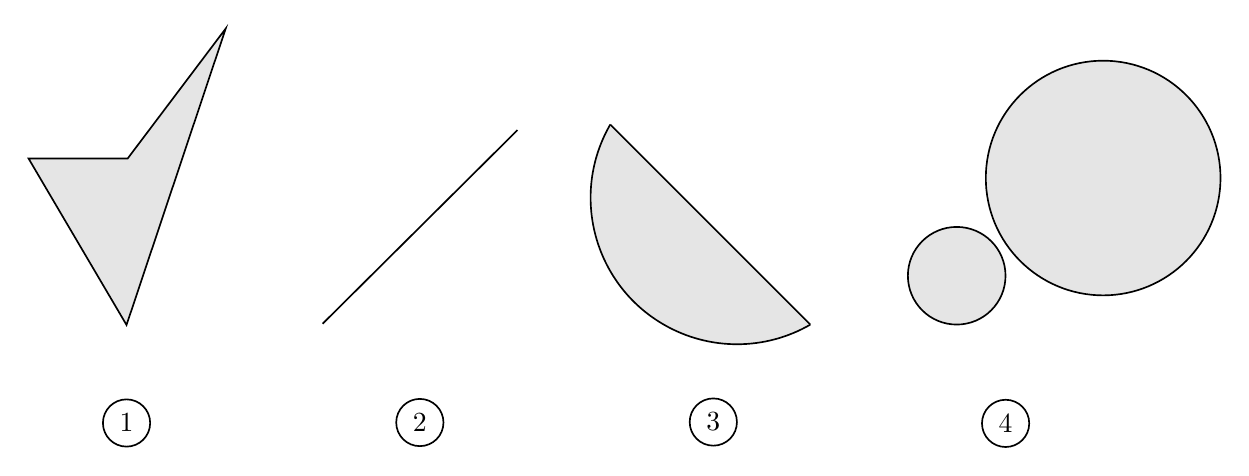
\begin{tikzpicture}[x=1cm,y=1cm,line width=.6pt,font=\normalsize]
\coordinate (FL) at (0.15,3.825);
\coordinate (FN) at (1.41,3.825);
\coordinate (FS) at (2.655,5.475);
\coordinate (FB) at (1.395,1.71);
\fill[gray!20] (FL)--(FN)--(FS)--(FB)--cycle;
\draw (FL)--(FN)--(FS)--(FB)--cycle;
\coordinate (FS1) at (3.885,1.725);
\coordinate (FS2) at (6.36,4.185);
\draw (FS1)--(FS2);
\coordinate (FC3) at (9.148,3.325);
\coordinate (FE1) at (7.538,4.255);
\coordinate (FE2) at (10.079,1.715);
\fill[gray!20] (FE1) arc[start angle=150,end angle=300,radius=1.86cm]--cycle;
\draw (FE1) arc[start angle=150,end angle=300,radius=1.86cm];
\draw (FE1)--(FE2);
\coordinate (FCS) at (11.938,2.335);
\coordinate (FCL) at (13.798,3.576);
\fill[gray!20] (FCS) circle[radius=0.62cm];
\draw (FCS) circle[radius=0.62cm];
\fill[gray!20] (FCL) circle[radius=1.49cm];
\draw (FCL) circle[radius=1.49cm];
\node[draw,circle,inner sep=0pt,minimum size=0.6cm] (N1) at (1.395,0.465) {1};
\node[draw,circle,inner sep=0pt,minimum size=0.6cm] (N2) at (5.12,0.471) {2};
\node[draw,circle,inner sep=0pt,minimum size=0.6cm] (N3) at (8.847,0.477) {3};
\node[draw,circle,inner sep=0pt,minimum size=0.6cm] (N4) at (12.559,0.46) {4};
\end{tikzpicture}
